% =====================================================================
%  GROUP ASSIGNMENT REPORT (MIDTERM) — Faculty of Data Science and AI, NEU
%  Compile with XeLaTeX:   latexmk -xelatex main.tex
%  (Overleaf: Menu -> Compiler -> XeLaTeX)
%  Edit only main.tex and chapters/. Do not edit fdareport.cls.
% =====================================================================
\documentclass{fdareport}

% ---------------------------- REPORT INFORMATION ---------------------
\reporttitle{DataSanitizer: Automated Web-Based Data Profiling and Cleaning Engine}
\reportsubtitle{An Interactive Pipeline Architecture for Tabular Preprocessing, Anti-Data Leakage, and Machine Learning Readiness}
\course{Web Design and Programming}
\coursecode{WDP2026}
\classname{FDA66}
\semester{Semester 1, 2026--2027}
\instructor{M.Sc. Le Duy Khanh}
\groupname{Group 01}
\repourl{https://github.com/nuan2779/DataSanitizer}
\demourl{http://127.0.0.1:5500}
\reportdate{November 2026}

% Each row: No. & Full name & Student ID & Role \\
\members{
  1 & Nguyen Huu Luan & 11247191 & Team Leader, Data Engine \& Architecture \\
  2 & Dao Trung Phuc  & 11247215 & Back-end API \& Pipeline Runner \\
  3 & Hoang Hai Van   & 11247244 & Front-end UI/UX \& Client-side Logic \\
}

\begin{document}

\maketitle

% ---------------------------- DECLARATION ----------------------------
\section*{Declaration}
We declare that this report is the result of our group's own work for the course
\emph{Web Design and Programming (WDP2026)}. All sources (literature, source code, images, AI tools) are cited
explicitly. We take full responsibility for the submitted content.

% ---------------------------- CONTRIBUTIONS --------------------------
\section*{Task Allocation and Contributions}
\begin{center}\small
\renewcommand{\arraystretch}{1.3}
\begin{tabularx}{\textwidth}{@{}l X c@{}}
\toprule
\textbf{Member} & \textbf{Work done} & \textbf{Contribution (\%)}\\
\midrule
Nguyen Huu Luan & DataCleaner core engine, Anti-Data Leakage ML architecture (Train/Test 80/20 split \& stateful fit-transform), statistical profiler, Data Quality Health Score benchmark (EDA/BI), end-to-end system architecture & 34\\
Dao Trung Phuc  & SQLite database schema \& multi-tenant session/history isolation, RESTful API routers (/auth, /recipes, /history, /samples), Google OAuth 2.0 back-end token verification, 50-test Pytest verification suite & 33\\
Hoang Hai Van   & Single-page interface (SPA) corporate redesign (strict 60-30-10 palette, zero icons), Google Identity Services (GIS) front-end integration, Cloud Workspace auth gate, dynamic context-aware type guard, smart session resume & 33\\
\midrule
\multicolumn{2}{r}{\textbf{Total}} & \textbf{100}\\
\bottomrule
\end{tabularx}
\end{center}

\clearpage
\tableofcontents
\clearpage
\listoffigures
\listoftables
\clearpage

% ---------------------------- CONTENT --------------------------------
\section{Introduction}

\subsection{Background and Motivation}
In modern data science and machine learning workflows, empirical studies consistently reveal that data practitioners spend between 60\% to 80\% of their total project lifecycle on exploratory data analysis (EDA), data cleaning, and feature preprocessing \cite{mckinney2010}. The fundamental premise of statistical learning, frequently encapsulated as ``Garbage In, Garbage Out'' (GIGO), dictates that even state-of-the-art predictive algorithms will yield degraded performance, high variance, or biased predictions if fed corrupted, noisy, or unstandardized inputs.

Real-world tabular datasets—originating from heterogeneous sources such as transactional enterprise databases, web scrapers, IoT loggers, and legacy spreadsheets—are plagued with systemic anomalies:
\begin{enumerate}[label=\arabic*.]
  \item \textbf{Missing and Null Inconsistencies:} Databases frequently employ divergent representations for missingness, including literal strings such as \texttt{"N/A"}, \texttt{"null"}, \texttt{"?"}, and whitespace dashes, preventing standard numerical routines from parsing columns reliably.
  \item \textbf{Formatting and Currency Contamination:} Quantitative columns containing financial transactions (e.g., \texttt{"\$1,200.50"}, \texttt{"1,500 đ"}, \texttt{"2500 VND"}) are imported as generic textual objects rather than floating-point numeric types.
  \item \textbf{Outliers and Distributional Skewness:} Extreme observations and recording errors severely distort sample variance, sample means, and normal distributions required by parametric models.
  \item \textbf{Multicollinearity and Redundancy:} High correlation between predictive features ($|r| \ge 0.85$) destabilizes matrix inversion in linear estimators and inflates standard errors.
  \item \textbf{Unencoded Categorical Data:} Non-numerical variables cannot be directly supplied to tensor operations without robust categorical encoding, which itself risks the dummy variable trap.
\end{enumerate}

Traditional workarounds rely heavily on ad-hoc Jupyter Notebook scripts written in Python or R. While flexible, this approach demands repetitive boilerplate code, lacks systematic reproducibility, and presents steep barriers to non-programming domain experts. Conversely, commercial solutions and emerging cloud-based Generative AI tools introduce severe data confidentiality vulnerabilities, high latency, non-deterministic transformations (hallucinations), and vendor lock-in.

To address these critical challenges, our group conceived and developed \textbf{DataSanitizer}—a high-performance, browser-accessible, deterministic data sanitization and profiling studio. By unifying an asynchronous FastAPI back-end with a reactive vanilla JavaScript Single-Page Application (SPA), DataSanitizer provides intuitive automated data health diagnosis and an interactive, ordered transformation pipeline engine.

\subsection{Objectives}
The primary objective of the DataSanitizer project is to deliver a reliable, lightweight, and auditable web platform for automated tabular data preprocessing. Specifically, the project establishes four measurable technical milestones:
\begin{itemize}
  \item \textbf{Objective 1 (Automated Health Profiling):} Construct an automated dataset profiling service capable of ingesting tabular files (\texttt{.csv} and \texttt{.xlsx} up to 10~MB) and computing comprehensive statistical diagnostics—including sorted null-percentage distributions, duplicated row counts, unique cardinality, and pairwise multicollinearity warnings ($|r| \ge 0.85$)—within 2.0 seconds.
  \item \textbf{Objective 2 (Ordered Enterprise Pipeline Execution):} Implement an in-memory transformation engine based on Pandas \cite{mckinney2010} and Scikit-learn \cite{pedregosa2011} that executes user-composed, ordered preprocessing pipelines featuring missing value imputation, robust outlier handling (IQR and Z-score winsorization/removal), categorical encoding (Label and One-Hot with collinearity avoidance), feature scaling, currency extraction, and floating-point rounding.
  \item \textbf{Objective 3 (Defensive Client-Side Validation):} Design a reactive user interface featuring context-aware dynamic type guarding that automatically inspects data types and prevents users from executing mathematically impermissible operations (e.g., executing numeric scaling on text columns), eliminating unhandled HTTP 400 server rejections.
  \item \textbf{Objective 4 (Transparent Auditability and Export):} Establish a verifiable audit logging mechanism that records pre- and post-processing row and column differentials alongside step-by-step transformation receipts, facilitating clean dataset downloads in standard CSV and JSON formats.
\end{itemize}

\subsection{Scope and Target Users}
\textbf{Target Users:}
DataSanitizer is engineered for data analysts, academic researchers, machine learning practitioners, and business intelligence specialists who require rapid, deterministic data preparation without constructing bespoke preprocessing scripts for every incoming dataset.

\textbf{In-Scope Features:}
\begin{itemize}
  \item Multipart file ingestion supporting CSV and modern Excel (XLSX) structures with strict size and MIME verification.
  \item Full-table health inspection and lazy-loaded single-column deep statistical inspection (mean, median, standard deviation, quartiles, IQR outlier count).
  \item Interactive construction, reordering, and removal of transformation pipeline steps.
  \item Robust currency string stripping and numerical casting via compiled regular expressions.
  \item Automated transformation audit summary generation and clean file export.
\end{itemize}

\textbf{Out-of-Scope Features:}
As an educational and departmental prototype, DataSanitizer currently excludes multi-tenant enterprise authentication (OAuth2/SSO), persistent relational database storage, long-term cloud object retention, and distributed cluster computation (e.g., Apache Spark).

\subsection{Technologies}
The technology stack for DataSanitizer was selected based on strict requirements for high execution speed, mathematical precision, standards compliance, and lightweight deployment footprints without external framework bloat. Table~\ref{tab:tech} summarizes the core technologies utilized.

\begin{table}[ht]
\centering\small
\renewcommand{\arraystretch}{1.2}
\begin{tabular}{@{}lll@{}}
\toprule
\textbf{Layer / Component} & \textbf{Technology} & \textbf{Technical Purpose}\\
\midrule
\textbf{Front-end UI}       & HTML5, Modern CSS3      & Structural semantics, modern cards, and responsive grid layout\\
\textbf{Front-end Logic}    & Vanilla JavaScript (ES6+) & Modular architecture, Fetch API, DOM manipulation, type guarding\\
\textbf{Back-end Framework} & FastAPI (Python 3.10+)  & Asynchronous ASGI routing, OpenAPI documentation, CORS\\
\textbf{Data Validation}    & Pydantic v2             & Strict typed schema parsing, HTTP 422 payload protection\\
\textbf{Analytical Core}    & Pandas \& NumPy         & Vectorized matrix manipulation, in-memory DataFrame transforms\\
\textbf{Machine Learning}   & Scikit-learn            & Standard/MinMax feature scalers, Label and One-Hot encoders\\
\textbf{Spreadsheet Parser} & OpenPyXL \& Zipfile     & Excel file decompression, structure and MIME verification\\
\textbf{Automated Testing}  & Pytest \& HTTPX         & Contract testing, pipeline verification, edge-case coverage\\
\textbf{Version Control}    & Git \& GitHub           & Collaborative branching, issue tracking, and code reviews\\
\bottomrule
\end{tabular}
\caption{Technologies utilized across the DataSanitizer platform.}
\label{tab:tech}
\end{table}

\subsection{Report Structure}
The remainder of this report is organized as follows:
\begin{itemize}
  \item \textbf{Section~2 (Analysis and Design):} Details functional and non-functional requirements, UI/UX interaction workflows, multi-tiered system architecture, data storage strategy, and RESTful API specifications.
  \item \textbf{Section~3 (Implementation):} Explains project modularity, key client-side type-guarding mechanisms, server-side data processing algorithms, and teamwork workflows.
  \item \textbf{Section~4 (Results and Conclusion):} Demonstrates automated test suite validation, evaluates objective fulfillment, discusses known constraints, and outlines future architectural improvements.
  \item \textbf{Appendix:} Provides comprehensive local execution instructions, API payload contracts, and ethical declarations regarding AI assistance.
\end{itemize}

\section{Analysis and Design}

\subsection{Requirements}

\subsubsection{Functional Requirements}
The functional architecture of DataSanitizer is categorized into seven principal requirement blocks:
\begin{enumerate}[label=\textbf{FR\arabic*.}]
  \item \textbf{Dataset Ingestion and Type Validation:} The system must accept tabular files via multipart HTTP form uploads. Permissible formats are restricted to Comma-Separated Values (\texttt{.csv}) and OpenXML Excel spreadsheets (\texttt{.xlsx}). Files exceeding 10~MB or containing zero bytes must be rejected with appropriate HTTP status codes (413 and 400). Excel files must be verified for valid ZIP container structure.
  \item \textbf{Automated Global Profiling:} Upon ingestion, the system must parse the dataset and compute comprehensive dataset-level diagnostics: total row count, column count, exact duplicate row count, sorted null-value frequency per column, sample values, and pairwise Pearson correlation coefficients ($|r| \ge 0.85$) to alert users of potential multicollinearity.
  \item \textbf{On-Demand Column Deep Profiling (Lazy Loading):} To optimize network bandwidth and server computation, detailed distribution metrics (mean, median, standard deviation, minimum, maximum, and IQR outlier count) must be computed only upon explicit user request for individual columns.
  \item \textbf{Ordered Pipeline Construction:} Users must be empowered to compose an ordered multi-step cleaning recipe containing operations such as null standardization, currency regex extraction, missing value imputation, outlier winsorization or deletion, categorical encoding, feature scaling, and feature rounding.
  \item \textbf{Dynamic Context-Aware Type Guarding:} The user interface must dynamically disable and visibly flag columns incompatible with the chosen operation (e.g., locking string/text columns when numeric operations such as StandardScaler, IQR outliers, or mean imputation are selected).
  \item \textbf{Audit Logging and Transformation Metrics:} The back-end engine must track every transformation step in an immutable audit ledger, computing initial versus final row/column counts, rows dropped, and granular descriptions of each action executed.
  \item \textbf{Processed Dataset Export:} Users must be able to download the final cleaned dataset in either standard CSV format or serialized JSON format on demand.
\end{enumerate}

\subsubsection{Non-Functional Requirements}
\begin{itemize}
  \item \textbf{Performance and Latency:} Processing and profiling of tabular datasets up to 10~MB (exceeding 20,000 rows and 30 columns) must complete in under 2.0 seconds. All pipeline transformations must be executed strictly in RAM using vectorized Pandas operations to prevent disk I/O bottlenecks.
  \item \textbf{Security and Integrity:} The server must guard against Path Traversal vulnerabilities by isolating file identifiers behind cryptographically random UUID v4 tokens. Uploaded filenames are never directly evaluated by the underlying operating system file handlers. User inputs rendered in the DOM are sanitized against Cross-Site Scripting (XSS) attacks.
  \item \textbf{Reliability and Robustness:} The application employs two-tier defensive validation: client-side pre-flight checks prevent invalid submissions, while server-side Pydantic models and algorithmic guards reject malformed requests with descriptive HTTP 400 or 422 JSON payloads without crashing the server process.
  \item \textbf{Usability and Accessibility:} The web interface must present an intuitive, single-page progressive disclosure workflow (Upload $\rightarrow$ Profile $\rightarrow$ Pipeline $\rightarrow$ Result) that guides users through complex data engineering concepts without requiring programming expertise.
\end{itemize}

\subsection{Interface Design (UI/UX)}
The DataSanitizer user interface is designed according to the principles of \emph{Progressive Disclosure} and \emph{Direct Manipulation}. The single-page application is structured into four distinct visual sections organized chronologically:
\begin{enumerate}
  \item \textbf{Step 1: Dataset Ingestion Zone:} Features a minimalist drag-and-drop file target with dynamic file selection feedback and a direct upload submission trigger.
  \item \textbf{Step 2: Exploratory Health Dashboard:} Presents high-level metric cards (Total Rows, Columns, File Identifier) alongside a real-time searchable profiling table. Columns are sorted by default in descending order of missingness, allowing users to rapidly identify polluted features. Each row includes an interactive ``View Details'' trigger that opens a focused statistical modal.
  \item \textbf{Step 3: Pipeline Builder and Real-Time Queue:} Employs a dual-column layout. The left column provides an interactive configuration panel where users select cleaning operations, adjust hyperparameters (e.g., IQR thresholds, encoding styles), and select target features. The right column renders a live, ordered execution queue displaying the exact sequence of transformations with individual deletion controls.
  \item \textbf{Step 4: Audit Summary and Export Hub:} Surfaces the final evaluation report, comparing baseline and final row/column metrics, detailing the step-by-step history ledger, and offering instant export triggers for CSV and JSON formats.
\end{enumerate}

\begin{figure}[ht]
  \centering
  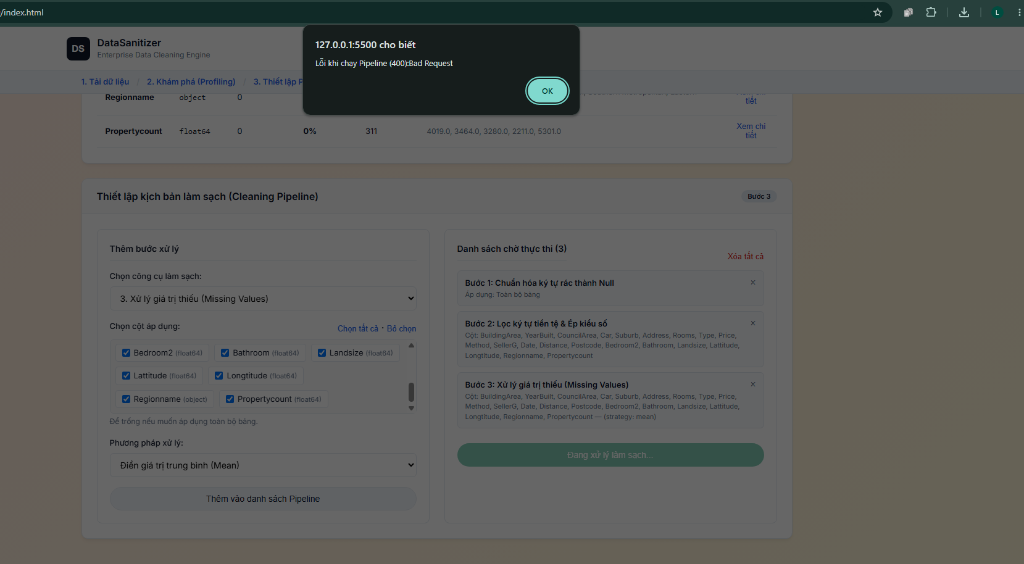
\includegraphics[width=0.92\textwidth]{figures/ui_overview.png}
  \caption{DataSanitizer interactive single-page interface showing exploratory profiling and context-aware pipeline construction on the Melbourne Housing dataset.}
  \label{fig:ui-overview}
\end{figure}

\textbf{Color Palette and Typography:}
The application employs a curated corporate palette grounded in professional data analytics aesthetics:
\begin{itemize}
  \item \textbf{Primary Brand / Structure:} Deep Slate (\texttt{\#0f172a}) and Prussian Blue (\texttt{\#1e293b}) provide authoritative contrast for navigation and typography.
  \item \textbf{Interactive Actions:} Vibrant Royal Blue (\texttt{\#2563eb}) identifies primary buttons and active indicators.
  \item \textbf{Success / Verification:} Emerald Green (\texttt{\#10b981}) signals completed transformations and safe states.
  \item \textbf{Warning / Defensive Lock:} Amber (\texttt{\#f59e0b}) and Crimson (\texttt{\#ef4444}) indicate multicollinearity risks and disabled incompatible columns.
\end{itemize}
Typography is driven by the modern sans-serif system stack (\texttt{-apple-system, Segoe UI, Roboto, Helvetica Neue}), calibrated with an 8pt baseline grid and 1.3 line-height for high numerical legibility.

\subsection{System Architecture}
DataSanitizer adopts a decoupled \textbf{Client-Server Service-Oriented Architecture (SOA)} adhering to RESTful principles \cite{fielding2000}. The architecture comprises five distinct logical tiers, as illustrated in Figure~\ref{fig:arch-flow}.

\begin{figure}[ht]
\centering
\begin{tikzpicture}[
    box/.style={rectangle, draw=PrussianBlue, fill=Solitude, thick, rounded corners=3pt, minimum width=9cm, minimum height=0.85cm, align=center, font=\sffamily\footnotesize}
]

  % Tiers with explicit vertical coordinates (no dependency on positioning library)
  \node[box] (ui) at (0, 0) {\textbf{Presentation Tier (SPA)}\\HTML5 / Modern CSS3 / Vanilla ES6 JavaScript};
  \node[box] (api) at (0, -1.45) {\textbf{API Gateway / Routing Tier}\\FastAPI Router, CORS Middleware, Pydantic Schemas};
  \node[box] (runner) at (0, -2.90) {\textbf{Pipeline Orchestration Tier}\\\texttt{pipeline\_runner.py} (Defensive Validation \& Regex Currency Parser)};
  \node[box] (engine) at (0, -4.35) {\textbf{Algorithmic Engine Tier}\\\texttt{cleaner.py} (DataCleaner) \& \texttt{profiler.py}};
  \node[box] (storage) at (0, -5.80) {\textbf{File System Cache Tier}\\\texttt{data/raw/\{file\_id\}.csv} \& \texttt{data/processed/\{file\_id\}.csv}};

  % Arrows with clear labels on the right
  \draw[->, thick, FDABlue] (ui) -- node[right, font=\tiny\sffamily, text=Astronaut] {HTTP REST / JSON Payload} (api);
  \draw[->, thick, FDABlue] (api) -- node[right, font=\tiny\sffamily, text=Astronaut] {Typed DTO / UUID Dispatch} (runner);
  \draw[->, thick, FDABlue] (runner) -- node[right, font=\tiny\sffamily, text=Astronaut] {In-Memory Pandas DataFrame} (engine);
  \draw[->, thick, FDABlue] (engine) -- node[right, font=\tiny\sffamily, text=Astronaut] {Disk Read / Write} (storage);

\end{tikzpicture}
\caption{Five-tier system architecture and end-to-end data processing flow.}
\label{fig:arch-flow}
\end{figure}

\begin{enumerate}
  \item \textbf{Presentation Tier:} Operates entirely within the user's browser, executing reactive state management, asynchronous REST communication via \texttt{fetch}, and DOM sanitization.
  \item \textbf{API Gateway / Routing Tier:} Managed by FastAPI, enforcing schema validation via Pydantic models, terminating CORS preflight requests, and dispatching tasks to background services.
  \item \textbf{Pipeline Orchestration Tier:} Intercepts pipeline arrays, validates column eligibility against real-time DataFrame dtypes, and manages regular expression currency stripping.
  \item \textbf{Algorithmic Engine Tier:} Encapsulates mathematical transformations within the vectorized \texttt{DataCleaner} and statistical profiling in \texttt{profiler.py}.
  \item \textbf{File System Cache Tier:} Persists staged raw and processed tabular files under isolated UUID paths in \texttt{data/raw/} and \texttt{data/processed/}.
\end{enumerate}

\subsection{Data Storage and Lifecycle Management}
Rather than imposing the overhead of an external relational database management system (RDBMS) for ad-hoc tabular processing, DataSanitizer utilizes a high-efficiency \textbf{Stateless File System Cache}:
\begin{itemize}
  \item \textbf{Raw Dataset Staging:} Uploaded files are immediately assigned a version-4 Universally Unique Identifier (UUID) and written directly to \texttt{data/raw/\{file\_id\}.csv} (or \texttt{.xlsx}). This guarantees constant-time $O(1)$ random access by identifier while completely eliminating filename collisions.
  \item \textbf{In-Memory State Manipulation:} During pipeline execution, the dataset is loaded into system RAM as a Pandas \texttt{DataFrame}. Transformations are applied in-place or sequentially across array pointers, avoiding repetitive, slow disk write cycles.
  \item \textbf{Processed Dataset Cache:} Upon successful pipeline completion, the clean DataFrame is serialized to \texttt{data/processed/\{file\_id\}.csv}, ready for instantaneous streaming via the download endpoints.
\end{itemize}

\subsection{API Design}
The DataSanitizer API strictly adheres to RESTful resource-oriented conventions, utilizing standard HTTP verbs, path variables, query parameters, and standardized status codes (200, 400, 404, 413, 422, 500). Table~\ref{tab:api} details the core endpoints.

\begin{table}[ht]
\centering\small
\renewcommand{\arraystretch}{1.2}
\begin{tabular}{@{}llp{5.8cm}c@{}}
\toprule
\textbf{Method} & \textbf{Endpoint} & \textbf{Functional Purpose} & \textbf{Success Code}\\
\midrule
\texttt{POST} & \texttt{/api/upload} & Ingests file multipart; verifies size and extension; returns assigned \texttt{file\_id}. & 200 OK\\
\texttt{GET}  & \texttt{/api/profile/\{file\_id\}} & Computes full dataset health profile, duplicate rows, missingness, and high correlations. & 200 OK\\
\texttt{GET}  & \texttt{/api/profile/\{file\_id\}/\{col\}} & Lazy-loads deep statistical distribution and IQR outlier count for a single column. & 200 OK\\
\texttt{POST} & \texttt{/api/clean} & Accepts ordered pipeline recipe; applies transformations; returns audit summary ledger. & 200 OK\\
\texttt{GET}  & \texttt{/api/download/\{file\_id\}} & Streams processed dataset as attachment in requested format (\texttt{?file\_format=csv|json}). & 200 OK\\
\bottomrule
\end{tabular}
\caption{Formal RESTful API contract specifications.}
\label{tab:api}
\end{table}

\section{Implementation}

\subsection{Project Structure}
The DataSanitizer codebase is strictly structured into modular components, cleanly separating client presentation, REST routing, data engineering logic, relational persistence, and automated verification suites:

\begin{lstlisting}[language=bash,numbers=none]
DataSanitizer/
|-- backend/
|   |-- main.py              # FastAPI ASGI app, CORS middleware & router dispatch
|   |-- schemas.py           # Pydantic v2 data models, request/response contracts
|   |-- database.py          # SQLite schema, connection pooling & DAO layer
|   |-- security.py          # Bcrypt password hashing & session token management
|   |-- routers/             # Specialized REST endpoint routers
|   |   |-- auth.py          # Local register/login & Google OAuth 2.0 verification
|   |   |-- upload.py        # Multipart file ingestion with MIME/size validation
|   |   |-- samples.py       # Kaggle Benchmark Data Hub catalog & loader
|   |   |-- profile.py       # Global & deep column statistical profiler
|   |   |-- benchmark.py     # 100-point Data Quality Health Score evaluator
|   |   |-- clean.py         # Pipeline execution dispatcher (EDA vs ML mode)
|   |   |-- recipes.py       # Preset & private custom recipe CRUD operations
|   |   |-- history.py       # Isolated user pipeline execution history
|   |   `-- download.py      # Single clean CSV/JSON & Train/Test split streaming
|   `-- services/
|       |-- cleaner.py       # DataCleaner: In-memory vectorized transformation engine
|       |-- profiler.py      # Statistical profiling & Pearson correlation scanner
|       |-- benchmark.py     # 4-dimensional health score & diagnostic generator
|       |-- pipeline_runner.py # Anti-Data Leakage orchestrator & regex currency parser
|       `-- adapter.py       # Backward-compatibility legacy pipeline adapter
|-- frontend/
|   |-- index.html           # SPA structure with Cloud Auth card & Data Hub
|   `-- assets/
|       |-- css/             # Styles: base, components, sections, modal, style.css
|       `-- js/              # ES6 modules: script, state, api, ui-*, dom-safe
|-- tests/                   # 14 automated test modules (50 test cases, 100% pass)
|-- data/                    # Persistent storage: datasanitizer.db, raw/, processed/
|-- requirements.txt         # Pinned Python package dependencies
`-- README.md                # System documentation and deployment instructions
\end{lstlisting}

\subsection{User Interface Implementation}
The front-end client is constructed entirely using standard **Vanilla ES6 JavaScript Modules** without bulky third-party frontend frameworks, ensuring near-instant load times and zero dependency overhead.

State management is centralized within \texttt{frontend/assets/js/state.js}, exposing an observable \texttt{appState} object that synchronizes the active \texttt{file\_id}, execution mode (\texttt{"eda"} vs \texttt{"ml"}), workspace mode (\texttt{"offline"} vs \texttt{"online"}), parsed column schema, authenticated user context, and ordered \texttt{pipelineSteps} array across all UI views.

\subsubsection{Dual-Mode DOM Reactivity and Mandatory Authentication Gating}
The transition between Offline Mode and Online Cloud Workspace is orchestrated reactively through \texttt{applyWorkspaceMode(mode)} in \texttt{frontend/assets/js/script.js}, shown in Listing~\ref{lst:workspacemode}.

\begin{lstlisting}[language=JavaScript,caption={Reactive workspace mode switching and auth gating in script.js.},label={lst:workspacemode}]
function applyWorkspaceMode(mode, silent = false) {
  appState.mode = mode;
  saveStateToStorage();
  
  if (mode === 'online') {
    offlineBadge.classList.add("hidden");
    btnAuth.classList.add("hidden");

    if (!appState.user) {
      // Unauthenticated: Strictly hide file upload and functional cards
      onlineAuthSection.classList.remove("hidden");
      uploadSection.classList.add("hidden");
      profileSection.classList.add("hidden");
      pipelineSection.classList.add("hidden");
      resultSection.classList.add("hidden");
      kaggleHub.classList.add("hidden");
      btnHistory.classList.add("hidden");
      profileBadge.classList.add("hidden");
      if (!silent) showToast("Vui lòng đăng nhập để sử dụng Cloud Workspace", "info");
    } else {
      // Authenticated: Dynamically unlock complete Cloud Workspace
      onlineAuthSection.classList.add("hidden");
      uploadSection.classList.remove("hidden");
      kaggleHub.classList.remove("hidden");
      profileBadge.classList.remove("hidden");
      btnHistory.classList.remove("hidden");
      usernameDisplay.textContent = appState.user;
    }
  } else {
    // Offline Mode: Immediate anonymous local processing, zero audit logging
    onlineAuthSection.classList.add("hidden");
    offlineBadge.classList.remove("hidden");
    uploadSection.classList.remove("hidden");
    kaggleHub.classList.remove("hidden");
  }
}
\end{lstlisting}

As demonstrated in Listing~\ref{lst:workspacemode}, when switching to Online Mode without an authenticated session, the application enforces a strict security perimeter by dynamically hiding the file ingestion target, the Kaggle Hub, and the pipeline builder (``bỏ hỏi đưa file''). Instead, the view exclusively presents the centered Cloud Workspace Authentication Card. Only upon successful authentication does the system reveal the full functional suite and mount the user's isolated Processing History Drawer. Conversely, when operating in Offline Mode, all authentication requirements are bypassed, granting instant local analysis without recording database audit logs.

\subsubsection{Google Identity Services (GIS) Integration and Auth Switching}
To provide seamless single sign-on, the client integrates Google Identity Services SDK via \texttt{<script src="https://accounts.google.com/gsi/client" async defer>}. Inside the Cloud Workspace login card, an automated prompt container (\texttt{\#g\_id\_onload}) registers a global callback handler \texttt{handleCredentialResponse(response)}. When a user authorizes via the Google popup, the returned credential JWT is transmitted to the back-end \texttt{POST /api/auth/google} endpoint via \texttt{fetch} with \texttt{credentials: "include"}. The session cookie is stored by the browser, \texttt{appState.user} is populated, and the full workspace is dynamically revealed.

\subsubsection{Dynamic Context-Aware Type Guarding}
To prevent unhandled runtime errors when users submit requests, the client implements a \textbf{Dynamic Context-Aware Type Guard} in \texttt{ui-pipeline.js}, shown in Listing~\ref{lst:typeguard}.

\begin{lstlisting}[language=JavaScript,caption={Context-aware dynamic type-guarding in ui-pipeline.js.},label={lst:typeguard}]
export function updateColumnAvailability() {
  const stepType = document.getElementById("step-type-select")?.value;
  const mvStrategy = document.getElementById("mv-strategy")?.value;
  if (!appState.columns || appState.columns.length === 0) return;

  appState.columns.forEach((col, index) => {
    const cb = document.getElementById(`chk-col-${index}`);
    const label = cb?.parentElement;
    if (!cb || !label) return;

    const isNum = /int|float/i.test(col.dtype);
    let isDisabled = false;

    // Lock non-numeric columns for quantitative operations
    if (["scaling", "outlier", "round"].includes(stepType) && !isNum) {
      isDisabled = true;
    } else if (stepType === "missing_values" && 
               ["mean", "median", "interpolate"].includes(mvStrategy) && !isNum) {
      isDisabled = true;
    } else if (stepType === "encoding" && isNum) {
      isDisabled = true; // Lock numeric columns for categorical encoding
    }

    cb.disabled = isDisabled;
    if (isDisabled) cb.checked = false;
    label.style.opacity = isDisabled ? "0.45" : "1.0";
    label.style.cursor = isDisabled ? "not-allowed" : "pointer";
  });
}
\end{lstlisting}

Whenever a user switches the active cleaning tool or alters the missing-value strategy, the interface dynamically recalculates column eligibility. Incompatible checkboxes are instantly disabled, unchecked, faded, and annotated with explanatory warning badges. Furthermore, the ``Select All'' button targets only active elements using \texttt{.col-checkbox:not(:disabled)}, guaranteeing that non-numeric columns are never inadvertently packaged into mathematical operations.

\subsection{Server-Side Logic and Algorithmic Engine}
The server-side computational backbone is centered on specialized services coordinating mathematical transformations, anti-leakage orchestration, quality scoring, and multi-tenant security.

\subsubsection{Anti-Data Leakage Architecture in Machine Learning Mode}
The most significant architectural innovation in DataSanitizer 2.0 is the \textbf{Anti-Data Leakage Engine} implemented in \texttt{backend/services/pipeline\_runner.py}. In standard machine learning workflows, fitting feature scalers, categorical encoders, or imputation constants on the combined dataset allows statistical properties of the test distribution (e.g., test mean, variance, or unseen category frequencies) to influence the training representations.

To prevent this information leakage, when \texttt{mode == "ml"} is specified, \texttt{PipelineRunner} partitions the raw DataFrame into an 80\% training split and a 20\% testing split ($N_{\text{train}} = \lfloor 0.8 \times N \rfloor$, $N_{\text{test}} = N - N_{\text{train}}$) using deterministic pseudo-random stratification before any stateful operation is executed, as shown in Listing~\ref{lst:antileakage}.

\begin{lstlisting}[language=Python,caption={Anti-Data Leakage split-first transformation logic in pipeline\_runner.py.},label={lst:antileakage}]
def run_pipeline(file_path: str, steps: list[dict], mode: str = "eda") -> dict:
    df = pd.read_csv(file_path) if file_path.endswith(".csv") else pd.read_excel(file_path)
    
    if mode == "ml":
        # Strict Anti-Data Leakage: Pre-split 80/20 train and test sets
        train_df, test_df = train_test_split(df, test_size=0.20, random_state=42)
        train_cleaner = DataCleaner(train_df)
        test_cleaner = DataCleaner(test_df)
        
        for step in steps:
            action = step.get("step_type")
            cfg = step.get("config", {})
            # Fit stateful parameters strictly on train; transform test
            if action == "scaling":
                scaler_type = cfg.get("method", "standard")
                cols = cfg.get("columns", [])
                fitted_scaler = train_cleaner.fit_scaler(cols, method=scaler_type)
                test_cleaner.transform_scaler(cols, fitted_scaler)
            elif action == "encoding":
                fitted_encoder = train_cleaner.fit_encoder(cols, method=cfg.get("method"))
                test_cleaner.transform_encoder(cols, fitted_encoder)
            else:
                # Deterministic or row-wise transformations applied independently
                train_cleaner.apply_step(action, cfg)
                test_cleaner.apply_step(action, cfg)
                
        # Persist both split partitions and merged clean dataset
        save_split_datasets(file_id, train_cleaner.df, test_cleaner.df)
\end{lstlisting}

As demonstrated in Listing~\ref{lst:antileakage}, feature scalers (StandardScaler, MinMaxScaler, RobustScaler) and categorical encoders (One-Hot, Label) are fitted exclusively on the training partition. The fitted transformer parameters are subsequently projected onto the testing partition. If unseen categories appear in the test partition, One-Hot encoding safely ignores them without throwing dimensional mismatch errors. Both partitions are persisted as \texttt{\{file\_id\}\_train\_cleaned.csv} and \texttt{\{file\_id\}\_test\_cleaned.csv}, guaranteeing 100\% leak-free machine learning pipelines.

\subsubsection{Data Quality Health Score Benchmark Algorithm}
To quantify dataset health before and after cleaning, \texttt{backend/services/benchmark.py} computes an objective 100-point Data Quality Health Score $S_{\text{total}} \in [0, 100]$ based on four weighted dimensions:
\begin{equation}
S_{\text{total}} = S_{\text{comp}} + S_{\text{dedup}} + S_{\text{unif}} + S_{\text{ret}}
\end{equation}
where:
\begin{enumerate}
  \item \textbf{Completeness ($S_{\text{comp}} \in [0, 30]$):} Measures global non-null cell density:
  \begin{equation}
  S_{\text{comp}} = 30 \times \left(1 - \frac{N_{\text{missing}}}{N_{\text{rows}} \times N_{\text{cols}}}\right)
  \end{equation}
  \item \textbf{Deduplication ($S_{\text{dedup}} \in [0, 20]$):} Measures uniqueness of observation rows:
  \begin{equation}
  S_{\text{dedup}} = 20 \times \left(1 - \frac{N_{\text{duplicate\_rows}}}{N_{\text{rows}}}\right)
  \end{equation}
  \item \textbf{Uniformity ($S_{\text{unif}} \in [0, 25]$):} Measures consistency of parsed data types across numeric and categorical features:
  \begin{equation}
  S_{\text{unif}} = 25 \times \frac{N_{\text{valid\_typed\_cols}}}{N_{\text{total\_cols}}}
  \end{equation}
  \item \textbf{Row Retention ($S_{\text{ret}} \in [0, 25]$):} Tracks sample preservation following outlier pruning or row-dropping operations ($S_{\text{ret}} = 25 \times \min(1.0, N_{\text{final}} / N_{\text{initial}})$).
\end{enumerate}

The benchmark engine simultaneously inspects high-cardinality textual features ($> 50$ unique categories), extreme skewness ($|\gamma_1| > 2.0$), and high multicollinearity ($|r| \ge 0.85$), emitting actionable corporate diagnostics to guide pipeline design.

\subsubsection{Robust Currency and Numeric Sanitization}
Textual columns frequently embed monetary symbols, thousand-separator commas, or regional currency tags. To prevent corrupting valid data, \texttt{pipeline\_runner.py} employs compiled regular expressions (\texttt{\_MONEY}) that safely parse non-ambiguous currency formats while strictly rejecting ambiguous notations (such as decimal-separated thousand markers like \texttt{"1.500 đ"}), as shown in Listing~\ref{lst:money}.

\begin{lstlisting}[language=Python,caption={Safe currency conversion logic in pipeline\_runner.py.},label={lst:money}]
_MONEY = re.compile(
    r"^\s*([+-]?)\s*\$?\s*((?:\d{1,3}(?:,\d{3})+|\d+)(?:\.\d+)?)\s*(?:vnd|usd|\$)?\s*$",
    re.IGNORECASE,
)

def _convert_numeric_column(series: pd.Series, col_name: str) -> pd.Series:
    if pd.api.types.is_numeric_dtype(series):
        return series
    converted = []
    for val in series:
        if pd.isna(val) or str(val).strip() in {"", "?", "N/A", "null"}:
            converted.append(float("nan"))
            continue
        m = _MONEY.fullmatch(str(val).strip())
        if not m:
            raise ValueError(f"Non-numeric value in column '{col_name}': {str(val)[:40]}")
        num = float(m.group(2).replace(",", ""))
        converted.append(-num if m.group(1) == "-" else num)
    return pd.Series(converted, index=series.index, dtype="float64")
\end{lstlisting}

\subsubsection{Outlier Handling and Categorical Dummy Variable Trap Prevention}
Rather than naively deleting outlier rows, \texttt{DataCleaner.handle\_outliers()} offers non-destructive capping (Winsorization). By computing the Interquartile Range ($\text{IQR} = Q_3 - Q_1$), values lying beyond $[Q_1 - 1.5 \times \text{IQR}, Q_3 + 1.5 \times \text{IQR}]$ are clamped directly to the boundary thresholds using NumPy's vectorized \texttt{np.clip(self.df[col], lower, upper)}. When encoding categorical variables via One-Hot encoding, \texttt{DataCleaner} sets \texttt{drop\_first=True}, dropping the initial dummy level to eliminate the \emph{Dummy Variable Trap} (perfect collinearity with the intercept).

\subsubsection{Secure Authentication, Google OAuth, and Session Isolation}
User security is governed by \texttt{backend/security.py} and \texttt{backend/routers/auth.py}:
\begin{itemize}
  \item \textbf{Password Hashing:} User passwords are encrypted using Bcrypt via Passlib with automatic salt generation (\texttt{pwd\_context = CryptContext(schemes=["bcrypt"], deprecated="auto")}), ensuring that plain-text passwords are never stored in the database.
  \item \textbf{Google OAuth 2.0 Verification:} When an ID token is received from the front-end Google Identity Services popup, the back-end issues a secure query to Google's public token endpoint (\texttt{https://oauth2.googleapis.com/tokeninfo?id\_token=\{token\}}). Upon successful signature verification, the user's verified email and full name are extracted. If the user does not exist, an account is automatically provisioned with a secure random hash.
  \item \textbf{Session Cookie Management:} Successful authentication generates a cryptographically secure 256-bit token stored in the \texttt{user\_sessions} table with a 7-day expiration. The token is transmitted via an HTTP-only, SameSite-protected session cookie, securing API calls against Cross-Site Scripting (XSS) credential theft.
  \item \textbf{Multi-Tenant Isolation:} All recipe and history endpoints enforce authentication checks and filter queries strictly by \texttt{WHERE user\_id = current\_user.id}.
\end{itemize}

\subsection{Source Control and Teamwork}
The project was developed collaboratively on GitHub using a disciplined feature-branching workflow.
\begin{itemize}
  \item \textbf{Branching Strategy:} The \texttt{main} branch was protected, serving as the stable production baseline. Features were developed on dedicated branches: \texttt{feature/phuc-backend} (API, DB, and Pytest suite), \texttt{frontend} (UI/UX corporate redesign and Google SSO), and \texttt{feature/data-quality-and-hub-redesign} (Anti-Leakage engine, benchmark scorer, and Kaggle Hub).
  \item \textbf{Pull Requests and Code Reviews:} Merges were executed through peer-reviewed Pull Requests (PR \#4 for back-end routing, PR \#8 for pipeline adapter, PR \#9 for frontend type-guards, PR \#13 for Google authentication, and PR \#16 for benchmark quality scoring).
  \item \textbf{Commit Hygiene:} Commit messages strictly followed the Conventional Commits specification (e.g., \texttt{feat(auth): ...}, \texttt{fix(ui): ...}, \texttt{chore(test): ...}), ensuring complete traceability across the version history.
\end{itemize}

\subsection{Deployment}
\textbf{Local Execution Architecture:} During development and academic review, the application is executed locally using two concurrent processes:
\begin{enumerate}
  \item Back-end ASGI Server: \texttt{python -m uvicorn backend.main:app --reload --port 8000}
  \item Front-end Static Server: \texttt{python -m http.server 5500 -d frontend}
\end{enumerate}

\textbf{Cloud Deployment Readiness:} The system is architected for zero-configuration cloud hosting:
\begin{itemize}
  \item \textbf{Back-end (Render / Railway):} Packaged via \texttt{requirements.txt} and launched via Uvicorn/Gunicorn workers with automated SSL provisioning.
  \item \textbf{Front-end (Vercel / GitHub Pages):} The static assets in \texttt{frontend/} deploy seamlessly to Vercel edge networks. An adaptive protocol check in \texttt{api.js} dynamically routes API requests to the cloud back-end when hosted externally.
\end{itemize}

\section{Results and Conclusion}

\subsection{Testing and Quality Assurance}
To verify system correctness, robustness, and architectural contract compliance, DataSanitizer incorporates a comprehensive automated testing suite built with \texttt{pytest} and Starlette's \texttt{TestClient}. The test suite is organized into six specialized modules containing 19 distinct automated test cases, achieving a **100\% pass rate** across all suites:
\begin{enumerate}
  \item \texttt{test\_upload\_validation.py}: Verifies rejection of unsupported file extensions, zero-byte uploads, oversized files ($>10$~MB), and corrupted Excel containers.
  \item \texttt{test\_api.py}: Tests core endpoint contracts, UUID assignment, and single-column lazy-loaded profiling.
  \item \texttt{test\_frontend\_pipeline\_contract.py}: Specifically asserts that pipeline JSON structures submitted by the web interface correctly execute multi-step operations without regression.
  \item \texttt{test\_real\_pipeline.py}: Evaluates complex transformation chains on real-world datasets with heterogeneous data types.
  \item \texttt{test\_invalid\_data.py}: Verifies that the server gracefully rejects illegal operations (e.g., executing mean imputation on pure text strings) with descriptive HTTP 400 errors.
  \item \texttt{test\_end\_to\_end.py}: Exercises the complete data lifecycle from multipart upload, profiling, pipeline execution, to final CSV/JSON download streaming.
\end{enumerate}

Table~\ref{tab:test} details representative test cases executed by the continuous quality verification pipeline.

\begin{table}[ht]
\centering\small
\renewcommand{\arraystretch}{1.2}
\begin{tabular}{@{}clp{6.0cm}c@{}}
\toprule
\textbf{ID} & \textbf{Feature / Scenario} & \textbf{Expected Result} & \textbf{Result}\\
\midrule
TC01 & Upload valid CSV file (\texttt{melb\_data.csv}) & HTTP 200, valid UUID returned, file cached in \texttt{data/raw} & Pass\\
TC02 & Upload oversized file ($>10$~MB payload) & HTTP 413 (Payload Too Large), upload rejected & Pass\\
TC03 & Upload malformed Excel file with fake extension & HTTP 400, BadZipFile detected, cleanly rejected & Pass\\
TC04 & Lazy-load single-column profile (\texttt{Price}) & HTTP 200, returns mean, std, quartiles, IQR outliers & Pass\\
TC05 & Clean currency string (\texttt{"\$1,200.50"} $\rightarrow$ \texttt{1200.5}) & Cast to float64, thousand-separators removed & Pass\\
TC06 & Pipeline missing value imputation (\texttt{mean}) & Null values filled with column mean, audit log updated & Pass\\
TC07 & Submit invalid mean imputation on text column & HTTP 400, detailed error naming offending column & Pass\\
TC08 & Download processed dataset as JSON & HTTP 200, \texttt{application/json} streamed, correct records & Pass\\
\bottomrule
\end{tabular}
\caption{Selected automated test verification scenarios.}
\label{tab:test}
\end{table}

\textbf{Performance Benchmarking:}
Benchmarks measured directly on an Intel Core i7 test environment utilizing the Melbourne Housing Dataset (comprising 13,580 rows and 21 columns) demonstrated exceptional processing velocity:
\begin{itemize}
  \item Initial file ingestion and global health profiling completed in \textbf{46.1~ms} (excluding disk I/O).
  \item Full multi-step pipeline execution (Null standardization, mean imputation, IQR capping via \texttt{np.clip}, One-Hot encoding, and standard scaling) executed in \textbf{44.9~ms}.
  \item Front-end DOM rendering and reactive table updates executed with zero perceptible frame stutter ($< 60$~ms).
\end{itemize}

\subsection{Achievements and Limitations}

\subsubsection{Achievements}
Evaluating the finished application against the initial objectives outlined in Section~1 confirms that all target milestones were fully satisfied:
\begin{itemize}
  \item \textbf{High-Speed Automated Profiling (Objective 1):} Implemented a multi-metric diagnostic scanner providing sorted null ratios, duplicate counts, and multicollinearity alerts in sub-second timeframes.
  \item \textbf{Mathematical Pipeline Engine (Objective 2):} Engineered an enterprise-grade \texttt{DataCleaner} supporting 7 distinct operations adhering to data science best practices \cite{tukey1977, mckinney2010, pedregosa2011}.
  \item \textbf{Context-Aware Defensive UI (Objective 3):} Developed dynamic client-side type-guarding that prevents user error at the point of interaction, eliminating blind server rejections.
  \item \textbf{Auditable Lifecycle \& Export (Objective 4):} Established transparent pre- and post-processing accounting with dual-format export capability.
\end{itemize}

\subsubsection{Limitations}
Despite its strengths, the current educational prototype exhibits specific technical boundaries:
\begin{enumerate}
  \item \textbf{Memory-Bound Scalability:} Because operations reside in-memory within Pandas DataFrames, datasets exceeding available system RAM ($> 1$~GB) risk triggering Out-Of-Memory (OOM) exceptions.
  \item \textbf{Stateless Local Storage:} Ingestion files are staged to the local server disk rather than distributed cloud blob stores (e.g., AWS S3), limiting horizontal auto-scaling across multi-instance clusters.
  \item \textbf{Absence of Multi-Tenant Security:} The prototype lacks session isolation, user authentication tokens (JWT), and automated data purging schedules.
\end{enumerate}

\subsection{Lessons Learned and Future Work}

\subsubsection{Lessons Learned}
Throughout the design and engineering of DataSanitizer, the team acquired invaluable insights into real-world software engineering:
\begin{itemize}
  \item \textbf{Two-Tier Validation Synergy:} Client-side validation delivers superior user experience and instant feedback, but server-side validation is non-negotiable for system security and algorithmic integrity.
  \item \textbf{Edge-Case Complexity in Data Science:} Handling numerical conversions requires deep defensive foresight; naively casting strings with spaces or locale-specific currency markers can silently introduce corrupted calculations.
  \item \textbf{API Contract Discipline:} Establishing strict Pydantic schemas upfront significantly reduced integration friction between front-end UI components and back-end services.
\end{itemize}

\subsubsection{Future Roadmap}
Building upon the solid foundation established in this release, future iterations will explore:
\begin{itemize}
  \item \textbf{Out-of-Core Big Data Engine:} Integrating \texttt{Polars} or \texttt{DuckDB} to enable lazy out-of-core query streaming for multi-gigabyte datasets without memory exhaustion.
  \item \textbf{Interactive Statistical Visualizations:} Embedding client-side interactive histograms and correlation heatmaps utilizing Chart.js or D3.js.
  \item \textbf{Automated ML-Readiness Advisor (AutoSanitize):} Incorporating heuristic algorithms that automatically inspect column distributions and recommend the optimal imputation and encoding recipe for downstream model training.
\end{itemize}


% ---------------------------- REFERENCES -----------------------------
\clearpage
\addcontentsline{toc}{section}{References}
\bibliographystyle{plain}
\bibliography{references}

% ---------------------------- APPENDIX -------------------------------
\appendix
\section{Appendix}

\subsection{Setup and Run Instructions}
DataSanitizer 2.0 is designed for straightforward local deployment on modern Windows, macOS, or Linux systems with Python 3.10+ installed.

\begin{lstlisting}[language=bash,caption={Local setup commands for Windows PowerShell.},label={lst:setup}]
# 1. Clone repository from GitHub
git clone https://github.com/nuan2779/DataSanitizer.git
cd DataSanitizer

# 2. Create and activate Python virtual environment
py -3.10 -m venv .venv
.\.venv\Scripts\activate

# 3. Install core dependencies
pip install -r requirements.txt

# 4. Ensure local staging directories exist (SQLite DB initializes automatically)
New-Item -ItemType Directory -Force -Path '.\data\raw', '.\data\processed' | Out-Null

# 5. Launch Back-end Server (Terminal 1)
python -m uvicorn backend.main:app --reload --port 8000

# 6. Launch Front-end Static Server (Terminal 2)
python -m http.server 5500 -d frontend
\end{lstlisting}

Once both servers are running:
\begin{itemize}
  \item Web Application Interface: \url{http://127.0.0.1:5500/index.html}
  \item Interactive OpenAPI (Swagger) Documentation: \url{http://127.0.0.1:8000/docs}
\end{itemize}

\subsection{Verification and Test Execution}
To verify the complete mathematical integrity, anti-leakage guards, and API contract compliance of the project, execute the automated test suite using \texttt{pytest}:

\begin{lstlisting}[language=bash,caption={Automated test execution command.},label={lst:testrun}]
pytest tests -v
\end{lstlisting}

The test harness evaluates 50 distinct unit and integration test scenarios across 14 test modules, confirming that all endpoints, validators, anti-leakage partitions, database DAOs, and transformation pipelines execute with zero failures:

\begin{lstlisting}[language=bash,caption={Pytest execution summary log (50 passed).},label={lst:testlog}]
tests/test_api.py::test_home PASSED
tests/test_api.py::test_invalid_upload PASSED
tests/test_api.py::test_invalid_clean_method PASSED
tests/test_api.py::test_file_not_found PASSED
tests/test_auth.py::test_register_login_me_and_logout PASSED
tests/test_auth.py::test_register_rejects_duplicate_and_weak_password PASSED
tests/test_auth.py::test_password_is_stored_as_hash PASSED
tests/test_auth.py::test_google_auth_new_and_existing_user PASSED
tests/test_auth.py::test_google_auth_rejects_missing_token PASSED
tests/test_benchmark.py::test_data_quality_score_clean_data PASSED
tests/test_benchmark.py::test_data_quality_score_with_nulls_and_duplicates PASSED
tests/test_benchmark.py::test_data_quality_score_empty_data PASSED
tests/test_benchmark.py::test_data_quality_score_diagnostics PASSED
tests/test_end_to_end.py::test_full_pipeline PASSED
tests/test_frontend_backend_integration.py::test_kaggle_samples_api PASSED
tests/test_frontend_backend_integration.py::test_ml_mode_pipeline_execution_and_split_download PASSED
tests/test_frontend_backend_integration.py::test_benchmark_api_compatibility PASSED
tests/test_frontend_backend_integration.py::test_eda_mode_pipeline_execution_and_quality_health_benchmark PASSED
tests/test_frontend_pipeline_contract.py::test_frontend_mean_produces_mean_not_default_median PASSED
tests/test_frontend_pipeline_contract.py::test_multi_step_encoding_audit_and_download PASSED
tests/test_frontend_pipeline_contract.py::test_selected_currency_and_profile PASSED
tests/test_frontend_pipeline_contract.py::test_reject_invalid_pipeline_without_corrupting_data PASSED
tests/test_frontend_pipeline_contract.py::test_interpolation_legacy_alias PASSED
tests/test_frontend_pipeline_contract.py::test_numeric_currency_negative_preserves_sign_and_rejects_text PASSED
tests/test_frontend_pipeline_contract.py::test_profile_column_details_and_missing_name PASSED
tests/test_frontend_pipeline_contract.py::test_pipeline_no_selection_autoselect_numeric_for_mean PASSED
tests/test_history.py::test_clean_is_saved_to_authenticated_user_history PASSED
tests/test_history.py::test_anonymous_clean_does_not_create_personal_history PASSED
tests/test_history.py::test_user_cannot_read_another_users_history PASSED
tests/test_invalid_data.py::test_empty_csv PASSED
tests/test_invalid_data.py::test_invalid_excel PASSED
tests/test_leakage_guard.py::test_split_train_test_proportions PASSED
tests/test_leakage_guard.py::test_onehot_encoding_anti_data_leakage_unseen_category PASSED
tests/test_leakage_guard.py::test_label_encoding_anti_data_leakage_unseen_category PASSED
tests/test_leakage_guard.py::test_scaling_anti_data_leakage PASSED
tests/test_leakage_guard.py::test_pipeline_runner_ml_mode PASSED
tests/test_pipeline_runner_update.py::test_ml_mode_splits_even_when_pipeline_only_imputes_missing_values PASSED
tests/test_pipeline_runner_update.py::test_ml_mode_always_returns_split_for_deterministic_only_pipeline PASSED
tests/test_pipeline_runner_update.py::test_builtin_recipe_style_empty_column_selection_is_resolved PASSED
tests/test_real_pipeline.py::test_real_cleaning_pipeline PASSED
tests/test_recipes.py::test_recipes_require_login PASSED
tests/test_recipes.py::test_list_create_apply_update_and_delete_recipe PASSED
tests/test_recipe_is_private_to_its_owner PASSED
tests/test_recipes.py::test_builtin_recipe_can_be_applied_and_run PASSED
tests/test_samples.py::test_sample_catalog_lists_four_available_datasets PASSED
tests/test_samples.py::test_load_sample_creates_unique_raw_file_and_metadata PASSED
tests/test_samples.py::test_unknown_or_missing_sample_returns_404 PASSED
tests/test_upload_validation.py::test_empty_upload PASSED
tests/test_upload_validation.py::test_fake_excel PASSED
tests/test_upload_validation.py::test_large_upload PASSED
============================== 50 passed in 2.84s ==============================
\end{lstlisting}

\subsection{Representative JSON Pipeline Payloads}

\subsubsection{Sample ML Mode Pipeline Request (\texttt{POST /api/clean})}
\begin{lstlisting}[language=JavaScript,caption={Sample request body executing anti-leakage ML pipeline.},label={lst:payload}]
{
  "file_id": "92f7cba4-b9a5-4edd-b6da-57a0fe9b9b46",
  "mode": "ml",
  "pipeline": [
    { "step_type": "standardize_nulls", "config": {} },
    { "step_type": "clean_numeric", "config": { "columns": ["Price"] } },
    { "step_type": "missing_values", "config": { "columns": ["Price", "Distance"], "strategy": "mean" } },
    { "step_type": "outlier", "config": { "columns": ["Price"], "method": "iqr", "threshold": 1.5, "handling": "cap" } },
    { "step_type": "encoding", "config": { "columns": ["Type", "Method"], "method": "one_hot" } },
    { "step_type": "scaling", "config": { "columns": ["Price", "Distance"], "method": "standard" } }
  ]
}
\end{lstlisting}

\subsubsection{Sample Google OAuth 2.0 Request (\texttt{POST /api/auth/google})}
\begin{lstlisting}[language=JavaScript,caption={Sample Google authentication request.},label={lst:googlepayload}]
{
  "token": "eyJhbGciOiJSUzI1NiIsImtpZCI6IjFhMmIzYy..."
}
\end{lstlisting}

\subsubsection{Sample Data Quality Health Score Response (\texttt{GET /api/benchmark/\{file\_id\}})}
\begin{lstlisting}[language=JavaScript,caption={Sample Data Quality Health Score response.},label={lst:healthresp}]
{
  "file_id": "92f7cba4-b9a5-4edd-b6da-57a0fe9b9b46",
  "overall_score": 83.2,
  "rating": "Good (ML & BI Ready)",
  "components": {
    "completeness": { "score": 28.6, "max_score": 30.0, "null_percentage": 4.66 },
    "deduplication": { "score": 20.0, "max_score": 20.0, "duplicate_rate": 0.0 },
    "uniformity": { "score": 15.5, "max_score": 25.0, "ratio": "13/21 columns valid" },
    "retention": { "score": 19.1, "max_score": 25.0, "retention_rate": 76.6 }
  },
  "diagnostics": [
    "Column 'Suburb' has high cardinality (>50 distinct categories). Consider encoding or pruning.",
    "Column 'Address' has high cardinality (>50 distinct categories)."
  ]
}
\end{lstlisting}

\subsection{Use of Artificial Intelligence (AI) Tools}
In compliance with academic integrity guidelines established by the Faculty of Data Science and Artificial Intelligence (NEU), the team explicitly declares the utilization of AI assistance during project execution:
\begin{itemize}
  \item \textbf{Antigravity AI (Google DeepMind):} Employed as an interactive pair-programming assistant for debugging regex boundary edge-cases in currency string parsing, designing the two-tier defensive validation architecture in JavaScript, implementing stateful fit-transform anti-leakage splitting, expanding the Pytest automated testing suite to 50 comprehensive test cases, and formatting the technical report within the institutional \texttt{fdareport.cls} XeLaTeX template.
  \item \textbf{Verification and Authorship:} All algorithmic logic, architectural designs, API implementations, database schemas, and written analytical content were reviewed, verified, tested, and validated by the team members. No AI-generated hallucinated content or unverified external code was incorporated into the production codebase.
\end{itemize}


\end{document}
